\documentclass{aip-cp}

\usepackage[numbers]{natbib}
\usepackage{rotating}
\usepackage{graphicx}
\usepackage{caption}

% Document starts
\begin{document}

% Title portion
\title{Light Meson Decays from Photon-Induced Reactions with CLAS}

\author[aff1]{Michael C. Kunkel\corref{cor1}}
\affil[aff1]{Forschungszentrum J\"ulich, J\"ulich (Germany)}
\corresp[cor1]{m.kunkel@fz-juelich.de}
\author{\textit{For the CLAS Collaboration}}
\maketitle

\begin{abstract}
Photo-production experiments with the CEBAF Large Acceptance Spectrometer (\textsc{\texttt{CLAS}}) at the Thomas Jefferson National Laboratory produce data sets with unprecedented statistics for light mesons. With these data sets, measurements of transition form factors for $\eta$, $\omega$, and $\eta^\prime$ mesons via conversion decays can be performed using the invariant mass distribution of the final state dileptons. Tests of fundamental symmetries and information on the light quark mass difference can be performed using a Dalitz plot analysis of the meson decay. An overview of the first results, from existing \textsc{\texttt{CLAS}} data, and future prospects within the newly upgraded \textsc{\texttt{CLAS12}} apparatus are given.
\end{abstract}

% Head 1
\section{INTRODUCTION}
Decays of light mesons provide insight into the structure of the meson. The Light Meson Decay (LMD) group, established at the Thomas Jefferson National Facility with worldwide collaboration, investigates physics pertaining to, but not limited to, transition form factors, anomalous decays and the search for CP violation through Dalitz plot analysis. The presentation given was an overview of the LMD program, recent updates on measurements and an outlook on measurements that can be taken with the \textsc{\texttt{CLAS12}} detector. 

\section{Light Meson Decay Program}
The light meson group was established in 2013. The goal of the group is to investigate properties of light meson decays using data obtained with the \textsc{\texttt{CLAS}} detector. Figure~\ref{fig:clas} shows the \textsc{\texttt{CLAS}} detector and its components.
\begin{figure}[h]
	\centerline{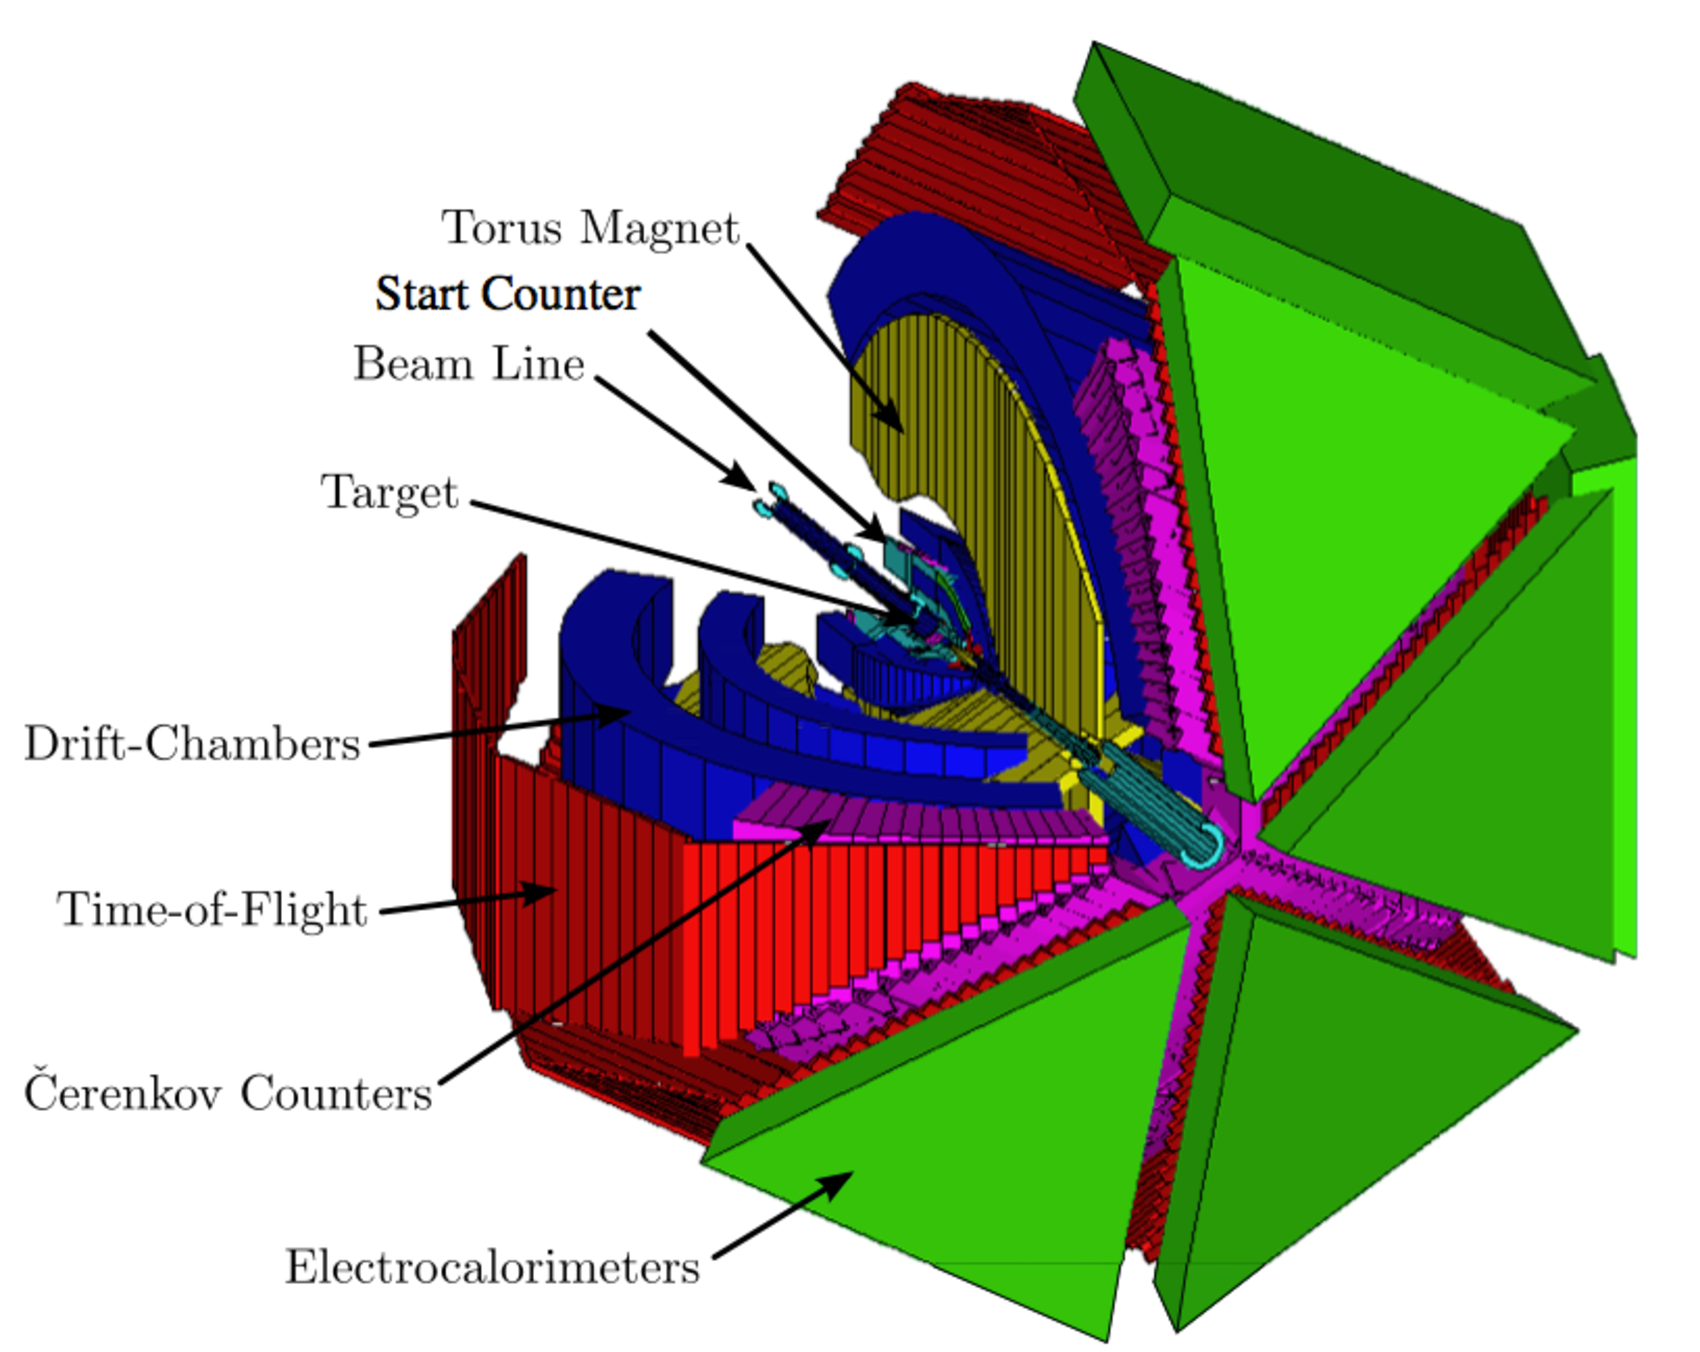
\includegraphics[width=175 pt]{figures/clas_schematicIII.pdf}}
	\caption{The CEBAF Large Acceptance Spectrometer (\textsc{\texttt{CLAS}}) }
	\label{fig:clas}
\end{figure}
 Since decays of hadrons are independent of production, all \textsc{\texttt{CLAS}} data can be used, however there are two experiments that were chosen as flagships for the program, the g11 and g12 experiment. Both experiments use a photon beam incident on a liquid hydrogen target which created photo-induced reactions with photon beam energies of 800~MeV - 3.8~GeV for g11 and 1.1~GeV - 5.5~GeV for g12.  See~\cite{lmdCAA} for a complete list of meson decays the LMD group plans to investigate.
% See Table~\ref{tab:lmd.channels} for a list of meson decays the LMD group plans to investigate.
%\begin{table}[h!]
\begin{minipage}{\textwidth}
\begin{center}


\caption{\label{tab:lmd.channels}LMD planned measurements \vspace{0.75mm}}
\begin{tabular}{cc||cc}
%\begin{tabular}{p{5cm} | p{7cm}}
\hline
Meson Decay & Physics Interest &Meson Decay & Physics Interest \\
\hline
$\pi^0\to e^+e^-\gamma$  & Heavy photon upper limit &$\eta^{\prime}\to \pi^+\pi^-\gamma$  & Box anomaly \\
$\eta^{\prime}\to e^+e^-\gamma$  & Transition form factor &$\omega\to \pi^+\pi^-\gamma$  & Upper limit branching ratio \\
$\omega\to e^+e^-\pi^0$ & Transition form factor & $\eta, \omega, \phi\to \pi^+\pi^-\pi^0$ & Dalitz plot analysis\\
$\eta^{\prime}\to e^+e^-\pi^0$ & C violation & $\eta^{\prime}\to \pi^+\pi^-\eta$ & Dalitz plot analysis\\
$\eta^{\prime}\to e^+e^-\pi^+\pi^-$  & CP violation & $\phi\to \pi^+\pi^-\eta$ & G-parity violation\\
\hline 
\end{tabular}


\end{center}
\end{minipage}
\end{table}
\vspace{20pt}
\subsection{The Radiative Decay of the $\eta$ and $\eta^\prime$  Meson}
The two-photon decay of the pseudoscalar mesons $\pi^0, \eta , \eta^{\prime} \to \gamma \gamma $ proceed via the triangle or axial anomaly. Radiative decays of  $\eta , \ \eta^{\prime} \to \pi^+ \pi^- \gamma $ are related to the box anomaly.
%\begin{figure}[h]
%	\begin{minipage}{.35\textwidth}
%		\centering
%		\centerline{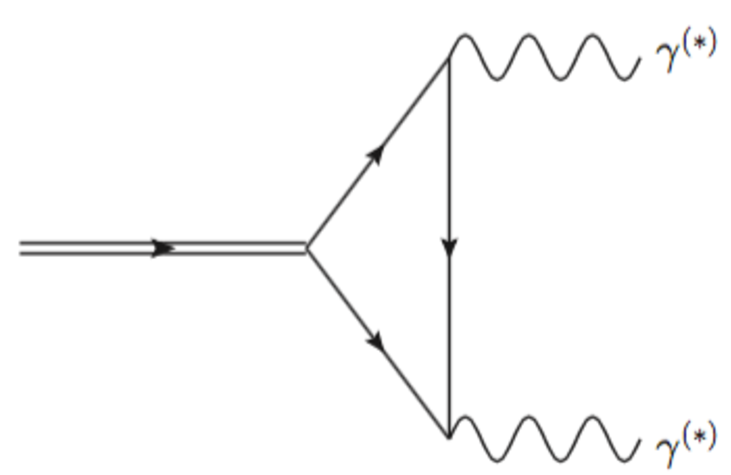
\includegraphics[width=75 pt]{figures/triangleIII.pdf}}
%		\caption{}{A. Triangle diagram}
%		\label{fig:test1}
%	\end{minipage}%
%	\begin{minipage}{.35\textwidth}
%		\centering
%		\centerline{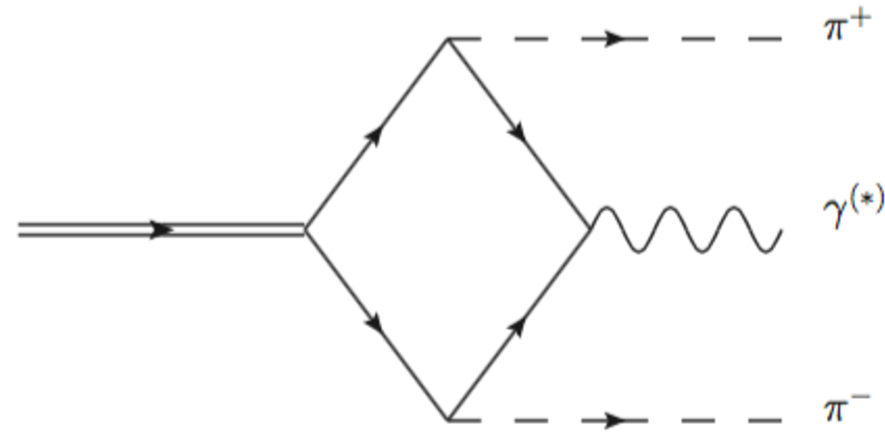
\includegraphics[width=75 pt, height=50 pt]{figures/boxIII.pdf}}
%		%\caption{figure in here}{box diagram}
%		\caption{Feynmann diagram of the two photon decay (A). Feynmann diagram of the axial anomoly, box diamgram (B)}{B. Box diagram}
%		\label{fig:decays}
%	\end{minipage}
%\end{figure}
The  radiative decay widths of $ \eta^{\prime}$ and $\eta^{\prime}$ are determined by the box anomaly in the chiral limit by Equation\ref{eq:decaywidth};

%An analysis of the photon energy distribution of the radiative decays of $ \eta^{\prime}$ and $\eta^{\prime}$, the decay widths are determined by the box anomaly in the chiral limit.

\begin{equation}

\frac{d\Gamma (\eta^{(\prime)} \to \pi^+ \pi^- \gamma)}{ds_{\pi\pi}} = A\vert P(s_{\pi\pi}) F_V(s_{\pi\pi}) \Gamma_0(s_{\pi\pi})\vert  \label{eq:decaywidth} \\

\end{equation}

where $\Gamma_0(s_{\pi\pi})$ is the P-wave phase-space constant, denoted in Equation~\ref{eq:decayconstant} with $\kappa$ being a numerical constant. $F_V(s_{\pi\pi})$ is the pion form factor that can be approximated by Equation~\ref{eq:decayformfactor} and  $P(s_{\pi\pi})$ is expanded around the chiral limit, $s_{\pi\pi} = 0$, as in Equation~\ref{eq:decaychiral}, where $\alpha$ is the variable of measurement.
\begin{eqnarray}
\Gamma_0(s_{\pi\pi}) = \frac{\kappa \left(M^2_{\eta^{(\prime)}} - s_{\pi\pi} \right)^3  s_{\pi\pi} \left(1- \frac{ 4M^2_{\pi }}{    s_{\pi\pi}  }\right)^{\frac{3}{2}}   }{M^3_{\eta^{(\prime)} }}  \label{eq:decayconstant}  \\
\vert F_V(s_{\pi\pi}) \vert \approx 1+(2.12\pm0.01)s_{\pi\pi} + (2.13\pm0.01)s_{\pi\pi}^2+(13.89\pm0.14)s_{\pi\pi}^3 \label{eq:decayformfactor} \\ \nonumber
\\ 
P(s_{\pi\pi}) = 1 + \alpha s_{\pi\pi} + \mathcal{O}(s_{\pi\pi}^2) \label{eq:decaychiral}
\end{eqnarray}
Previous results on the radiative decay for the $\eta$ meson from WASA-at-COSY~\cite{bib0} and KLOE~\cite{bib1} would profit from further measurements. Only one measurement exists for the $\eta^{\prime}$ radiative decay~\cite{bib2}. With the \textsc{\texttt{CLAS}} g11 experiment, both the $\eta$ and  $\eta^{\prime}$ radiative decay width will be measured. In Figure~\ref{fig:boxCLASdata} the \textsc{\texttt{CLAS}} g11 data is shown for the particle selection of exclusive $\gamma p \to p  \pi^+ \pi^- \gamma $. Selecting events within a $2.5 \sigma$ range of $\eta^{(\prime)}$ the photon energy distribution, which is related to $s_{\pi\pi}$ by Equation~\ref{eq:spipi}, is shown in Figure~\ref{fig:boxCLAS}. 

\begin{equation}

s_{\pi\pi} = m^2 - 2E_{\gamma}m \label{eq:spipi} \\

\end{equation}
\begin{figure}[h]
	\centerline{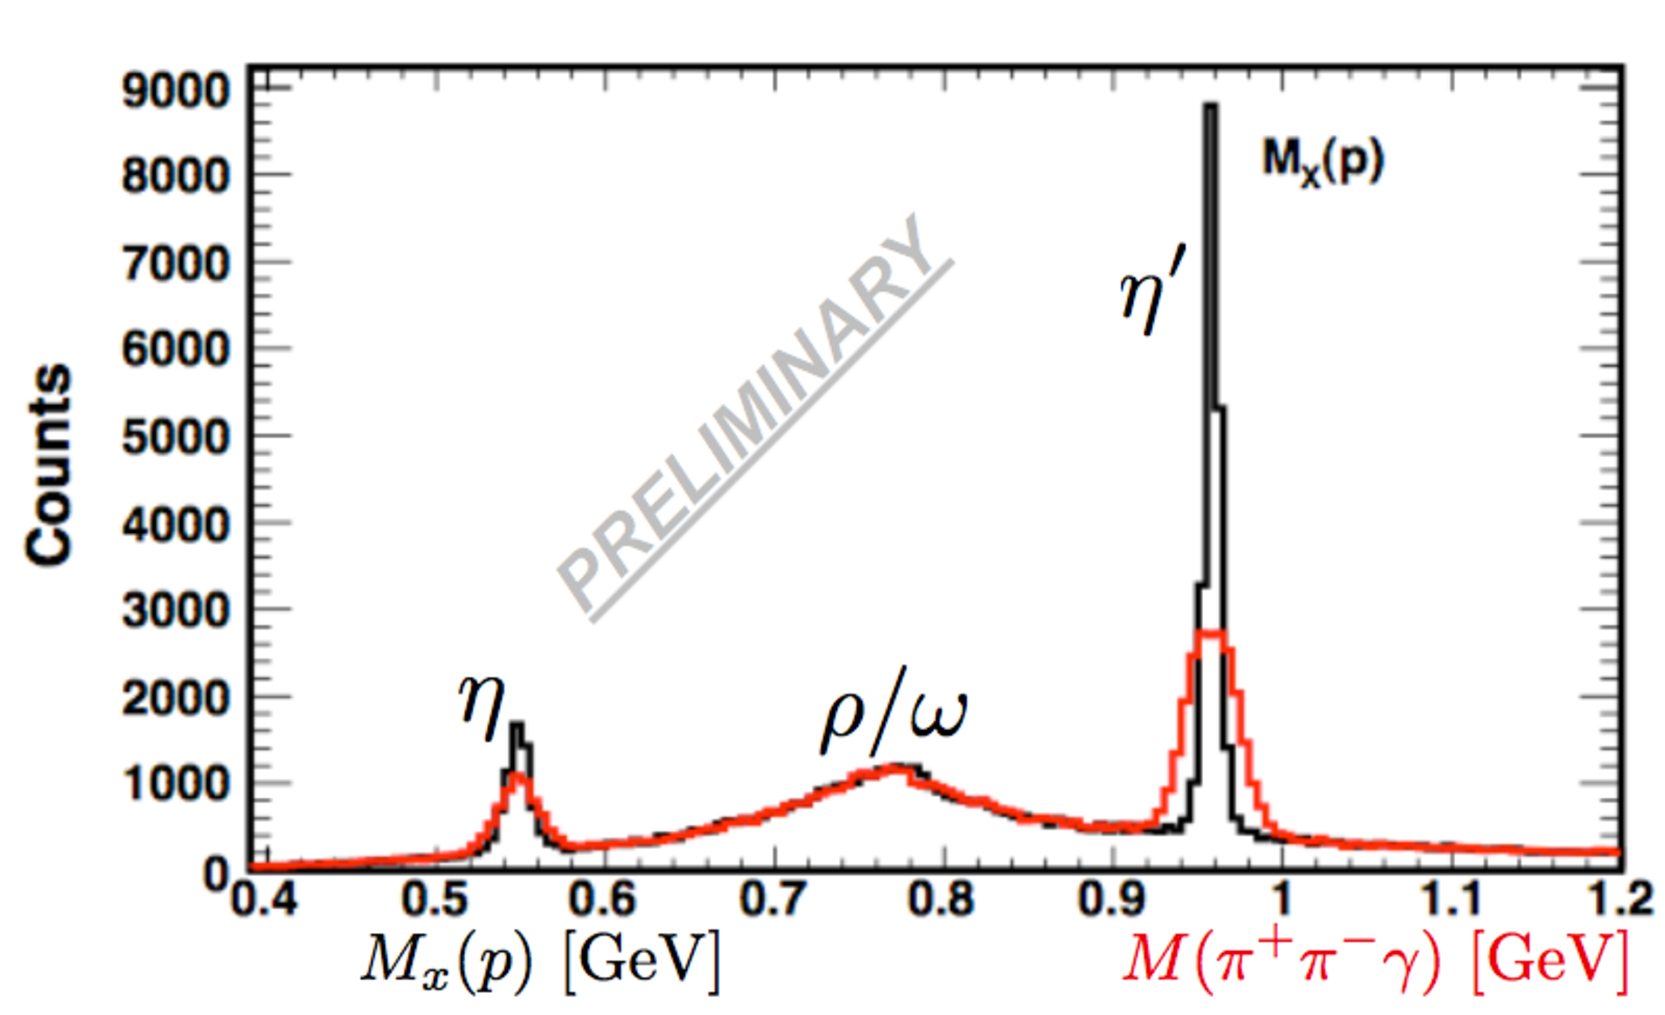
\includegraphics[width=275 pt, height = 200 pt ]{figures/clas_g11data.pdf}}
	\caption{\textsc{\texttt{CLAS}} yield for $\gamma p \to p \eta^{(\prime)} \to p \pi^+ \pi^- \gamma $ from the g11 data set }
	\label{fig:boxCLASdata}
\end{figure}
\begin{figure}[h]
	\centerline{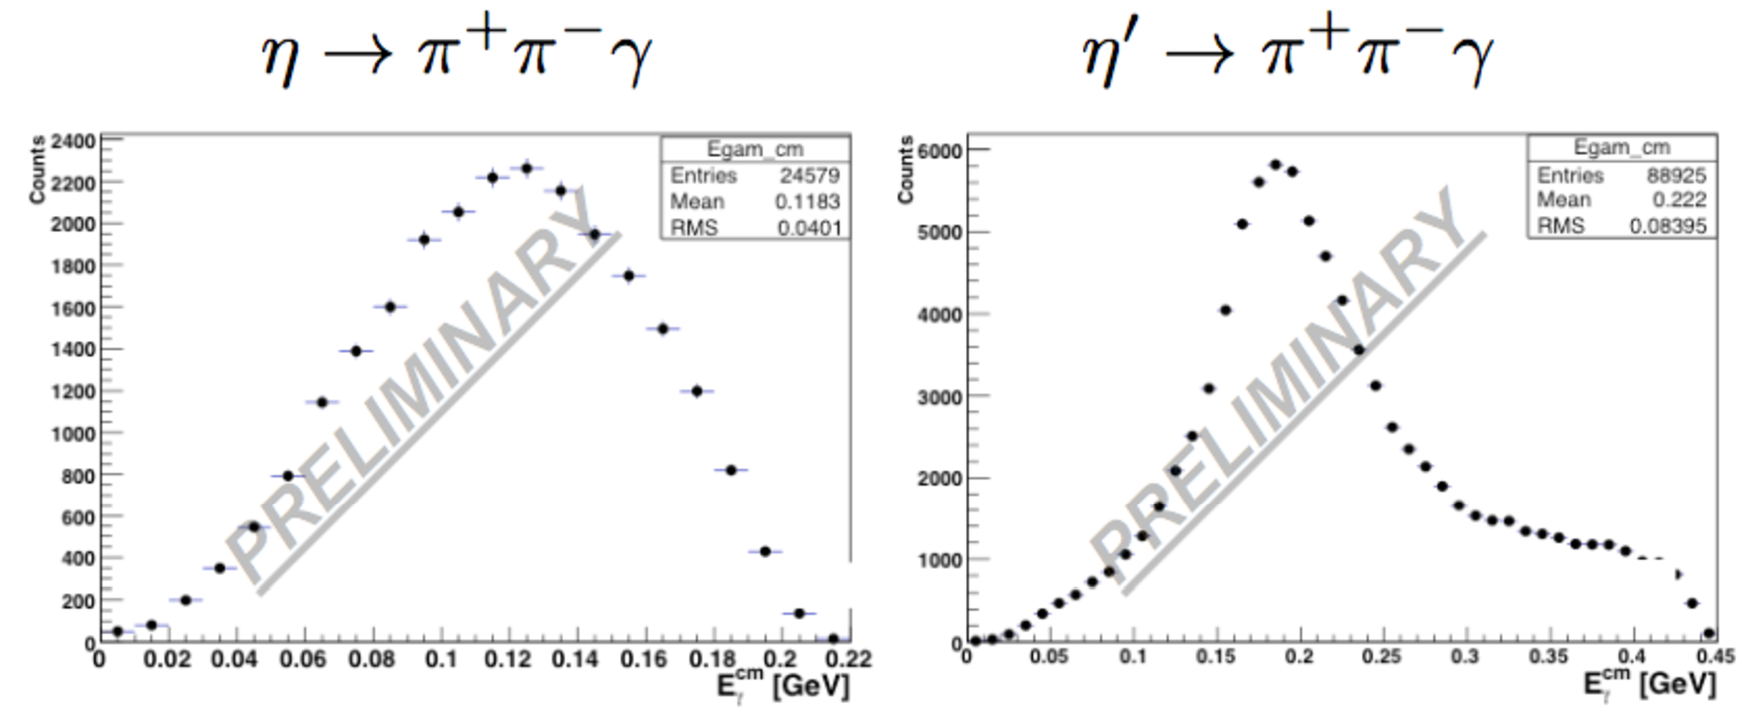
\includegraphics[width=275 pt]{figures/Box_CLAS.pdf}}
	\caption{\textsc{\texttt{CLAS}} photon energy distribution for $\eta$ (left) and $\eta^{\prime}$ (right)}
	\label{fig:boxCLAS}
\end{figure}
Comparing the shape of the left Figure~\ref{fig:boxCLAS} to those of Figure~\ref{fig:kloe_eta}, for the  $\eta$ meson, and also the right Figure~\ref{fig:boxCLAS} to that of Figure~\ref{fig:crystal_etaP}, for the $\eta^{\prime}$ meson, it can be seen that the \textsc{\texttt{CLAS}} data is suitable for comparison with previous measurements.
\begin{figure}[h!]
	\centering
	\begin{minipage}{.30\textwidth}
		\centering
		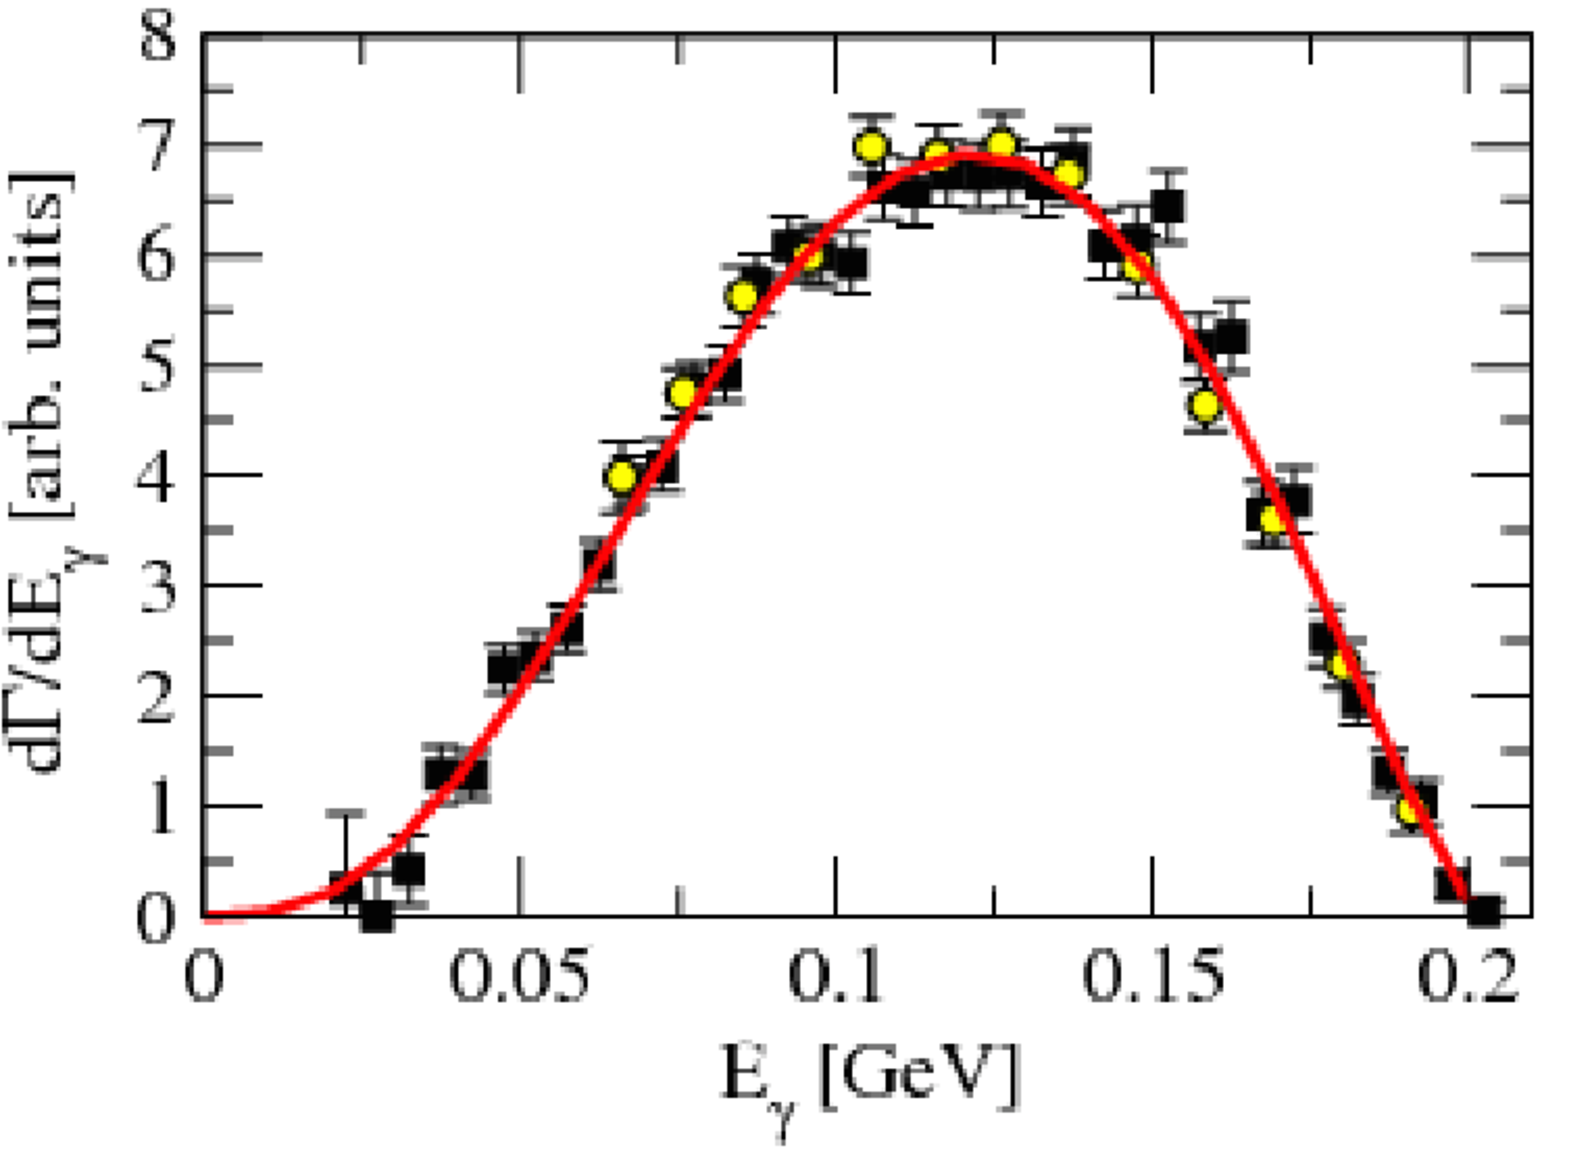
\includegraphics[width=125 pt]{figures/WASA_eta.pdf}
		\caption{}{}
		\label{fig:wasa_eta}
	\end{minipage}%
	\centering
	\begin{minipage}{.30\textwidth}
		\centering
		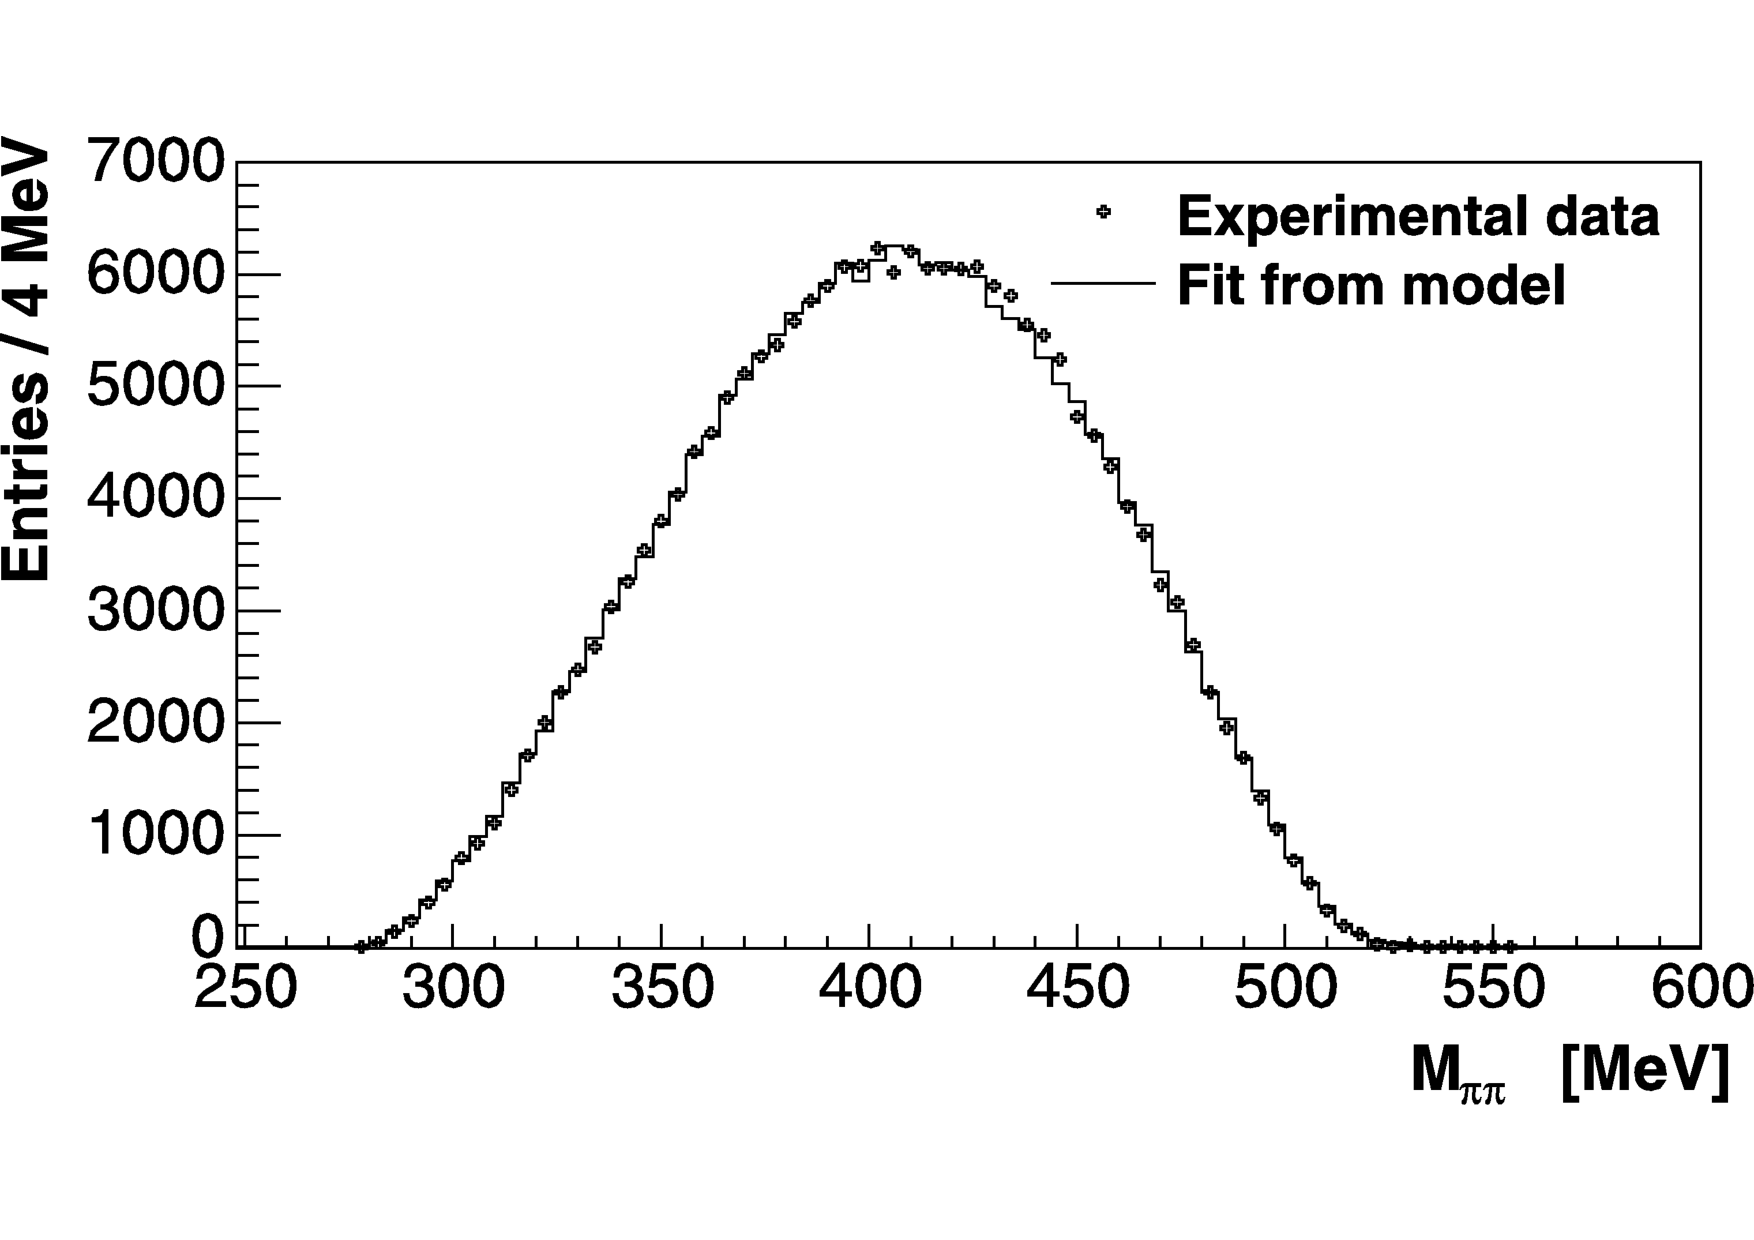
\includegraphics[width=125 pt, height = 100 pt]{figures/KLOE_eta.pdf}
		%\caption{figure in here}{box diagram}
		\caption{Left: Photon energy distribution for $\eta$ with model~\cite{bib3} ,showing the WASA-at-COSY data~\cite{bib0} (solid symbols) and previous results from ~\cite{grom} (yellow symbols). Right: The KLOE photon energy distribution for $\eta$ \cite{bib1}.}{}
		\label{fig:kloe_eta}
	\end{minipage}
\end{figure}
\begin{figure}[h!]
	\centerline{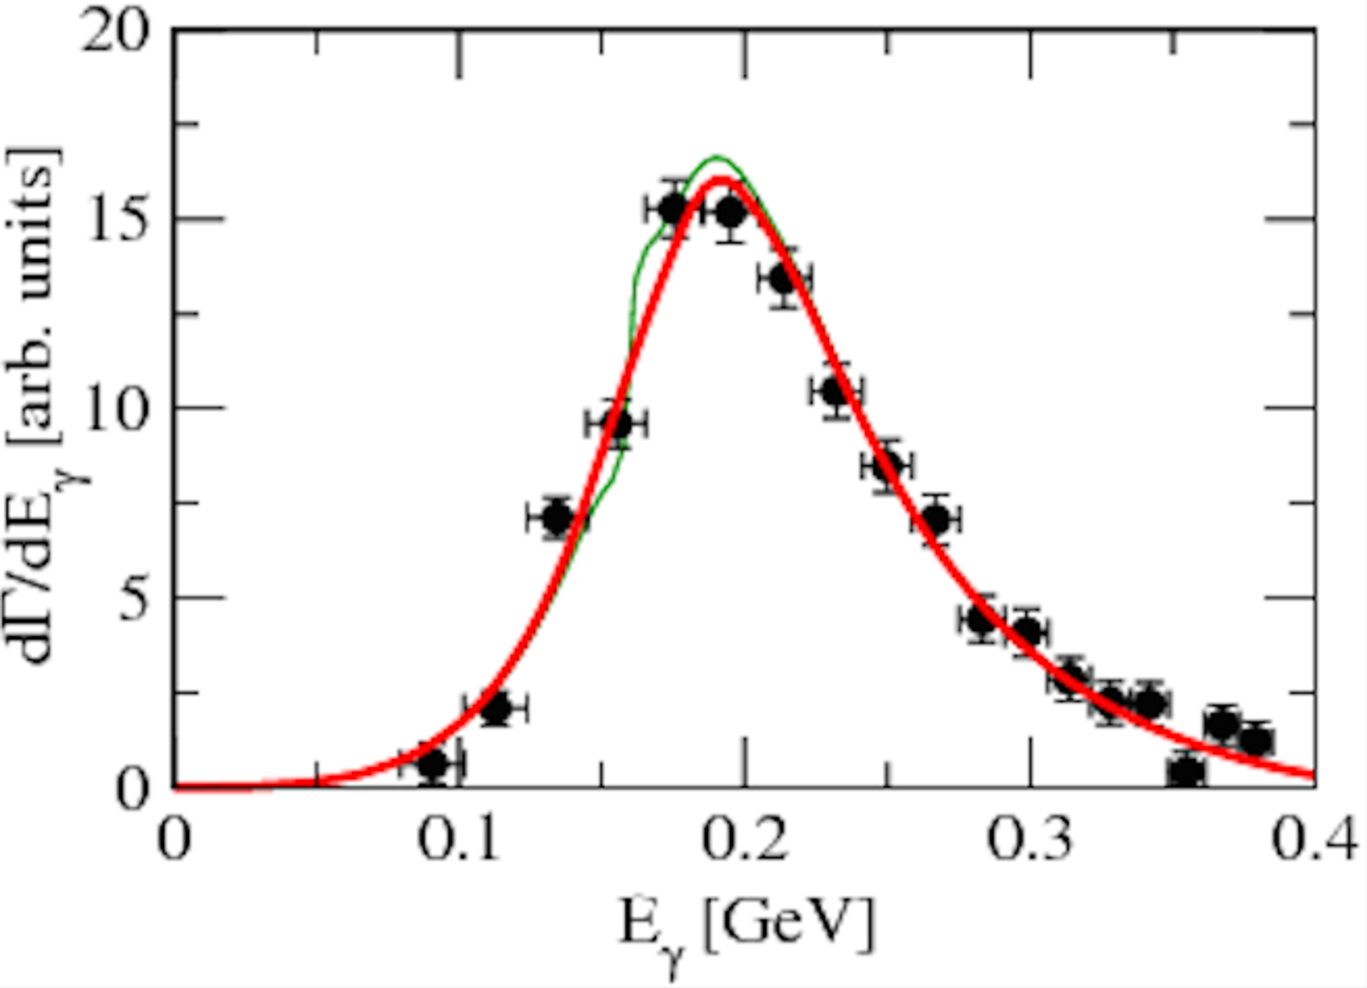
\includegraphics[width=135 pt]{figures/CRYSTAL_etaP.pdf}}
	\caption{CRYSTAL BARREL photon energy distribution for  $\eta^{\prime}$~\cite{bib2}}
	\label{fig:crystal_etaP}
\end{figure}
%\newpage
%\subsection{Update on the Dalitz plot analysis of $\eta^{\prime} \to \pi^+ \pi^- \eta$}
%%The Dalitz plot of $\eta^{\prime} \to \pi^+ \pi^- \eta$ provides kinematic information of the decay, enabling the study of low energy dynamics of QCD and heavier mass pseudoscalar mesons. The  $\eta^{\prime} \to \pi^+ \pi^- \eta$ decay has a low Q-value due to the decay products being relatively heavy, this helps test and limit the effective chiral Lagrangian theory. The measurable of the Dalitz plot $X$ and $Y$ are projected and fitted to the Equation~\ref{eq:dalitzpro} to extract the parameters $a$, $b$, $c$, $d$. Table~\ref{tab:dal.parms} shows the previous measurements of Equation~\ref{eq:dalitzpro} along with the projected statistical error a measurement from the CLAS g11 data.
%%
\begin{equation}
%%
f(X,Y) = A(1+a(Y) + b (Y^2) + c(X) + d(X^2)  \label{eq:dalitzpro} \\
%%
\end{equation}
%%
\begin{table}[h!]
\begin{minipage}{\textwidth}
\begin{center}


\caption{\label{tab:dal.parms}Previous \vspace{0.75mm}}
\begin{tabular}{cccccc}
%\begin{tabular}{p{5cm} | p{7cm}}
\hline
Parameter & VES & Theory & BESIII & Stat. err. in BESIII & Projected CLAS stat. err. \\
\hline
a & -0.127 $\pm$ 0.018 & -0.116 $\pm$ 0.011 & -0.047 $\pm$ 0.012 &$\pm$ 0.011&$\pm$ 0.004 \\
b & -0.106 $\pm$ 0.032 & -0.042 $\pm$ 0.034 & -0.069 $\pm$ 0.021 &$\pm$ 0.019&$\pm$ 0.006\\
c & 0.015                        &                                  & 0.019  $\pm$  0.012 &$\pm$ 0.011&$\pm$ 0.004\\
d & -0.082 $\pm$ 0.019 & -0.010 $\pm$ 0.019 & -0.073 $\pm$ 0.013 &$\pm$ 0.012&$\pm$ 0.004\\
\end{tabular}


\end{center}
\end{minipage}
\end{table}
\vspace{20pt}
%This topic was briefly discussed, as a full update was given by later in the session.
\subsection{The Transition Form Factor  of the $\omega$ Meson}
Transition form factors characterize modifications of the point-like photon-meson vertex due to the structure of the meson. The virtual photon can interact with quarks, therefore it can be used as a probe for the internal structure of mesons and its electromagnetic interaction is calculable with the Kroll-Wada formula~\cite{bib4}, Equation~\ref{eq:kroll};
\begin{equation}
\frac{d\Gamma_{M{\rightarrow l^{+}l^{-}X}}}{dq^{2} d\Gamma_{M{\rightarrow X\gamma}}} = \frac{\alpha}{3\pi q^{2}}\left(\left(1+\frac{q^{2}}{m^{2}_{M}-m^{2}_{X}}\right)^2 - \frac{4m^{2}_{M}q^2}{(m^{2}_{M}-m^{2}_{X})^2}\right)^\frac{3}{2}\left(1-\frac{4m_{l}^{2}}{q^{2}}\right)^{1/2}\left(1+\frac{2m_{l}^{2}}{q^{2}}\right) \bigg|_{\mathrm{Q.E.D}}  \label{eq:kroll} \ . \\
\end{equation}
 where $M$ is the species of meson i.e. $\pi^0$, $\eta$, $\omega$, $\eta^{\prime}$, etc., $X$ is the child particle in the decay, $m_M$ the mass of the meson, $m_X$ the mass of the child particle, $m_l$ the mass of the lepton species in the decay, i.e. $e^{\pm}$ or $\mu^{\pm}$ and $q$ being the momentum transfer which is identical to the invariant mass of the dilepton. Deviations of Equation~\ref{eq:kroll} represent the internal structure of the meson for pseudoscalar mesons, while for vector mesons the deviation represents the transition from $M \to X$. These deviations are the transition form factor $\left| F(q^2)\right|$ and can be determined by comparing Equation~\ref{eq:kroll} to what is measured experimentally.
 \begin{equation}
 \frac{d\Gamma_{M{\rightarrow l^{+}l^{-}X}}}{dq^{2} d\Gamma_{M{\rightarrow X\gamma}}}\bigg|_{\mathrm{measured}} =   \frac{d\Gamma_{M{\rightarrow l^{+}l^{-}X}}}{dq^{2} d\Gamma_{M{\rightarrow X\gamma}}} \bigg|_{\mathrm{Q.E.D}} \left| F(q^2)\right|^2 \label{eq:kroll_ff} \ . \\
 \end{equation}
 Depending on the decay width of the meson of interest, the transition can be modeled as a simple pole, Equation~\ref{eq:pole}, a complex pole, Equation~\ref{eq:cpole}, or some other function that describes the transition.
 \begin{eqnarray}
\left| F(q^2)\right| = \frac{1}{1-\frac{q^2}{\Lambda^2}} \label{eq:pole} \\
\left| F(q^2)\right|^2 = \frac{\Lambda^2(\Lambda^2 + \gamma^2)}{(\Lambda^2 - q^2)\Lambda^2 \gamma^2} \label{eq:cpole} \ ,
 \end{eqnarray} 
 where $\Lambda$ and $\gamma$ is the mass and width of the virtual vector meson mass, respectively.
 Recent measurements of the transition form factor for $\omega \to \mu^+\mu^- \gamma$ have shown unexpected discrepancies with the Vector Dominance Model~\cite{bib5} and recent models of chiral Lagrangian field theory~\cite{bib6}, and dispersion theory~\cite{Schneider} attempt to predict the contributions of the virtual vector meson as seen in Figure~\ref{fig:omega_ff}.
 \begin{figure}[h!]
 	\centerline{\includegraphics[width=250 pt, height=130 pt]{figures/omega_ff_bastian_edit.pdf}}
 	\caption{Form factor of the decay $\omega \to l^+l^- \gamma$ compared to dimuon data by the NA60 Collaboration~\cite{bib5,bib5_0} and LEPS~\cite{LEPS}. Shown are VMD (dotted line) Eqs.~(\ref{eq:kroll},~\ref{eq:cpole}) using the mass of the $\rho$ meson as the virtual vector meson, the results of a chiral Lagrangian treatment with explicit vector mesons~\cite{bib6} (white shaded curve with solid borders), a simplified approximation to the full dispersive solution~\cite{Schneider} (gray shaded curve with dashed borders), full dispersive solution~\cite{Schneider} (black hatched curve with solid borders).~\cite{Schneider}}
 	\label{fig:omega_ff}
 \end{figure}
 
With the \textsc{\texttt{CLAS}} g12 experiment, lepton ($e^{\pm}$) identification is done using Cherenkov detectors and electromagnetic calorimetry, providing a $e^{+}e^{-}/\pi^{+}\pi^{-}$ rejection of $10^6$. Using the $e^{\pm}$ data from \textsc{\texttt{CLAS}} g12, the $ \omega \to p e^+ e^- \pi^0$ transition form factor can be extracted. Figure~\ref{fig:clas_omega_ff} shows the region of the $\omega$ meson.
\begin{figure}[h!]
		\centering
		\centerline{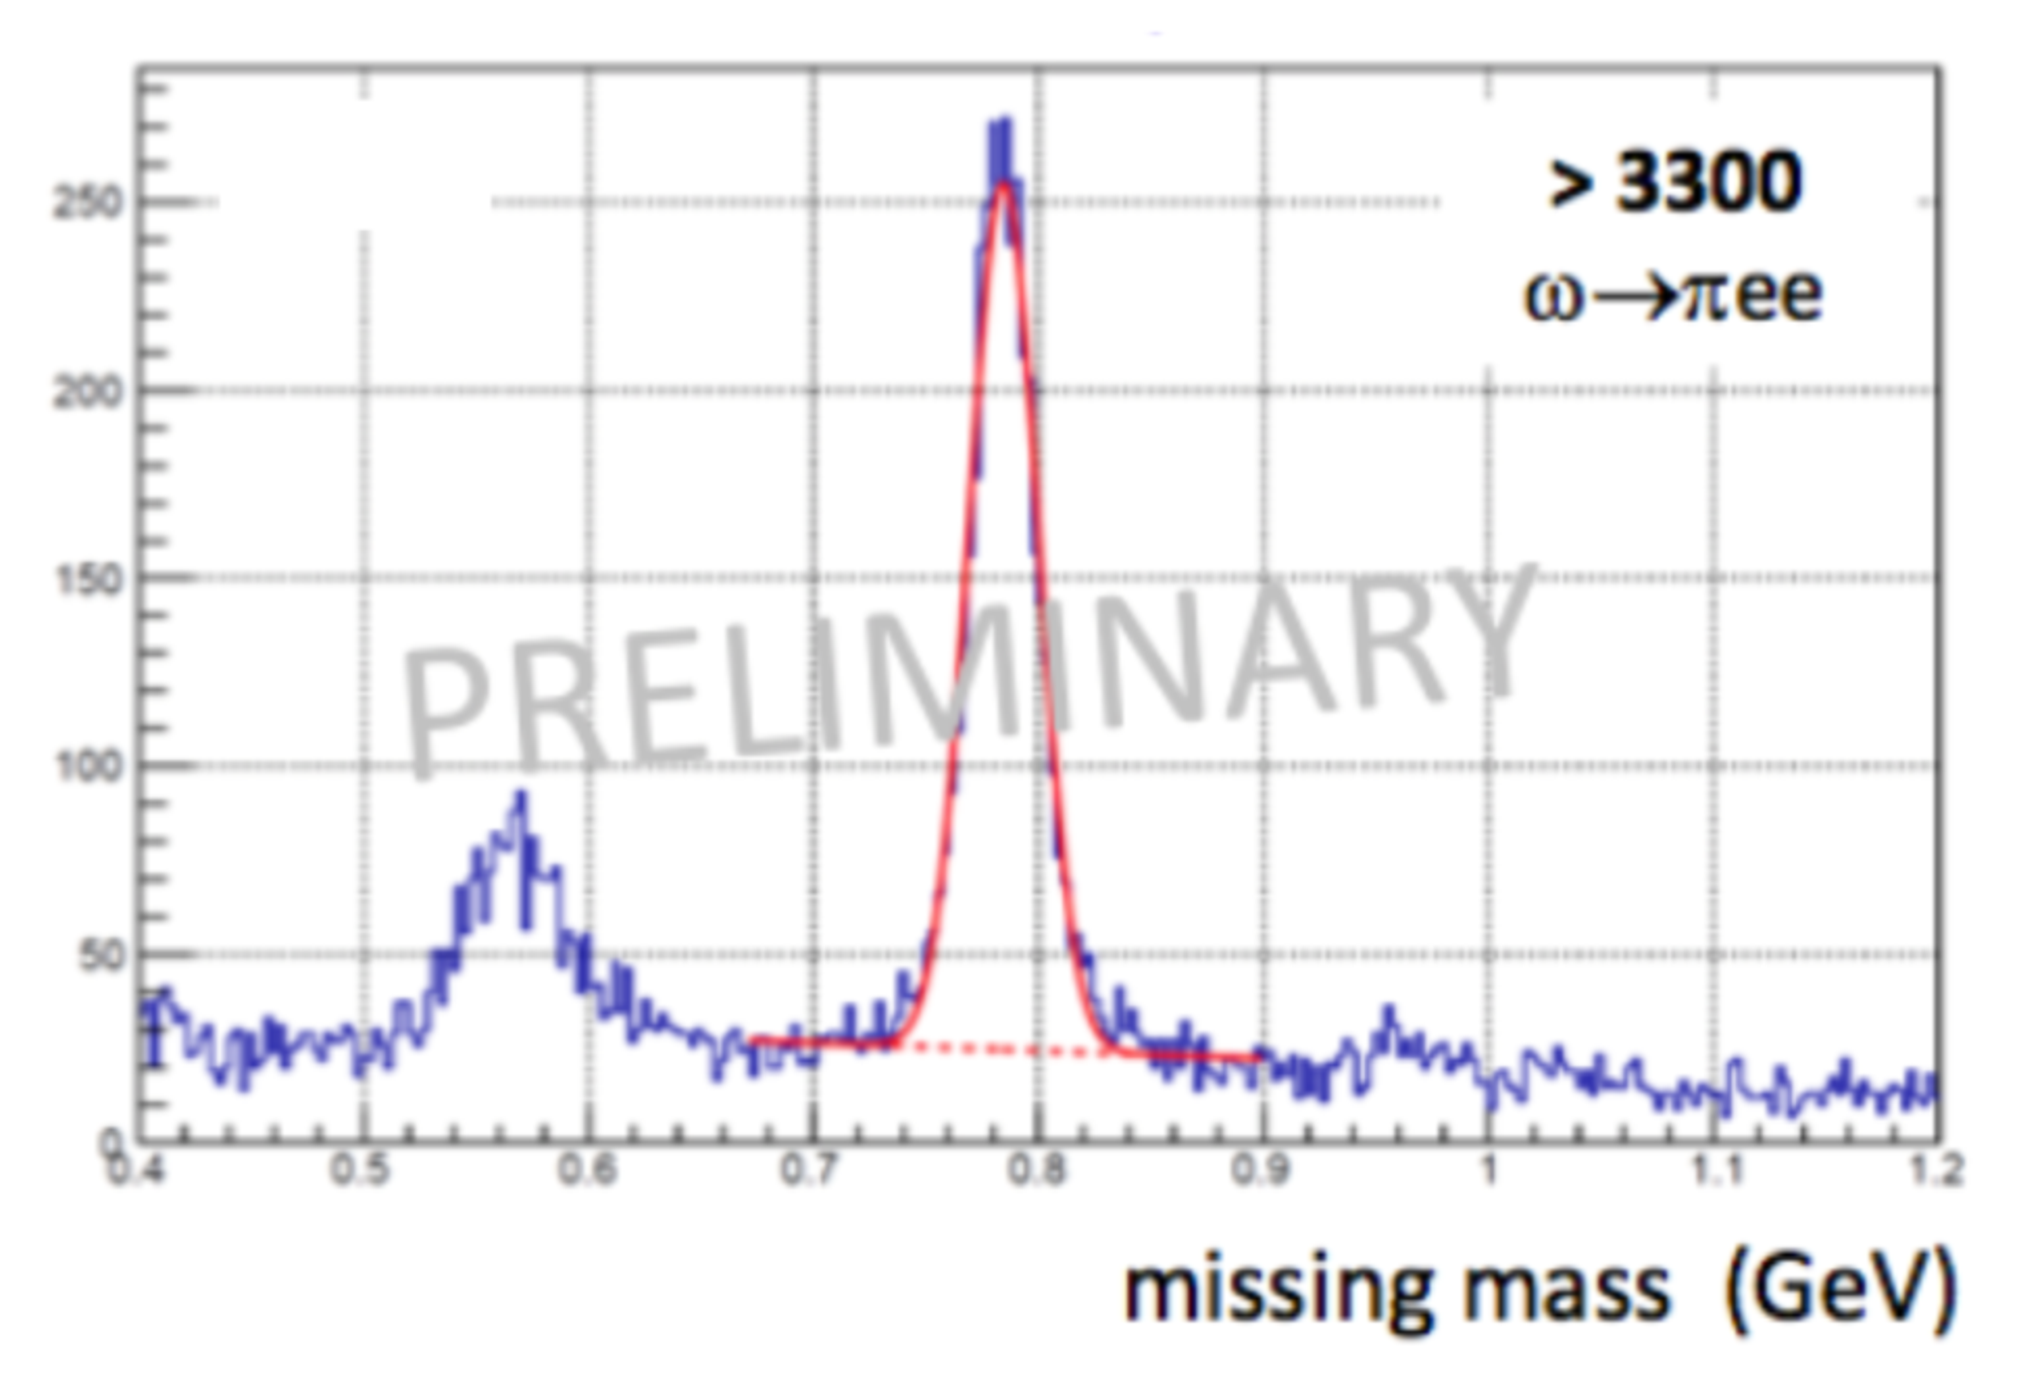
\includegraphics[width=150 pt]{figures/clas_omega_ff_II.pdf}}
		\caption{\textsc{\texttt{CLAS}} yield for $\gamma p \to p X \to p e^+ e^- \pi^0 $ from g12 data set}{}
		\label{fig:clas_omega_ff}
\end{figure}
Also, the knowledge of the $\eta$ form factor is needed for the interpretation of the $(g_{\mu}-2)/2$ uncertainty~\cite{gminus2}. Furthermore, the ratio of the $\eta$ and $\eta^{\prime}$ transition form factor provides information of the mixing angle of the combination of the singlet, $\eta_0$, and nonet, $\eta_8$, which are the components of the physical eigenstates, the $\eta$ and $\eta^{\prime}$ meson.
%\newpage
\subsection{Update on the Branching Ratio Measurement  of the $\eta^\prime \rightarrow e^+e^-\gamma$ Decay}
A recent measurement of BESIII reports the branching ratio $\Gamma(\eta^{\prime} \to  e^+ e^-  \gamma)$/$\Gamma(\eta^{\prime} \to  \gamma  \gamma)$ to be $2.13\pm0.09(stat.)\pm0.07(sys.))10^{-2}$ from 864 events~\cite{bib7}.  Using the $e^{\pm}$ data from \textsc{\texttt{CLAS}} g12, preliminarily 89 events of the $\eta^{\prime} \to  e^+ e^-  \gamma$ decay were observed and analyzed, using the Q-factor~\cite{bib8} method to suppress background from neighboring $A \to e^+ e^-  X$ decays, Figure~\ref{fig:etaP_ff}.
 \begin{figure}[h!]
 	\centerline{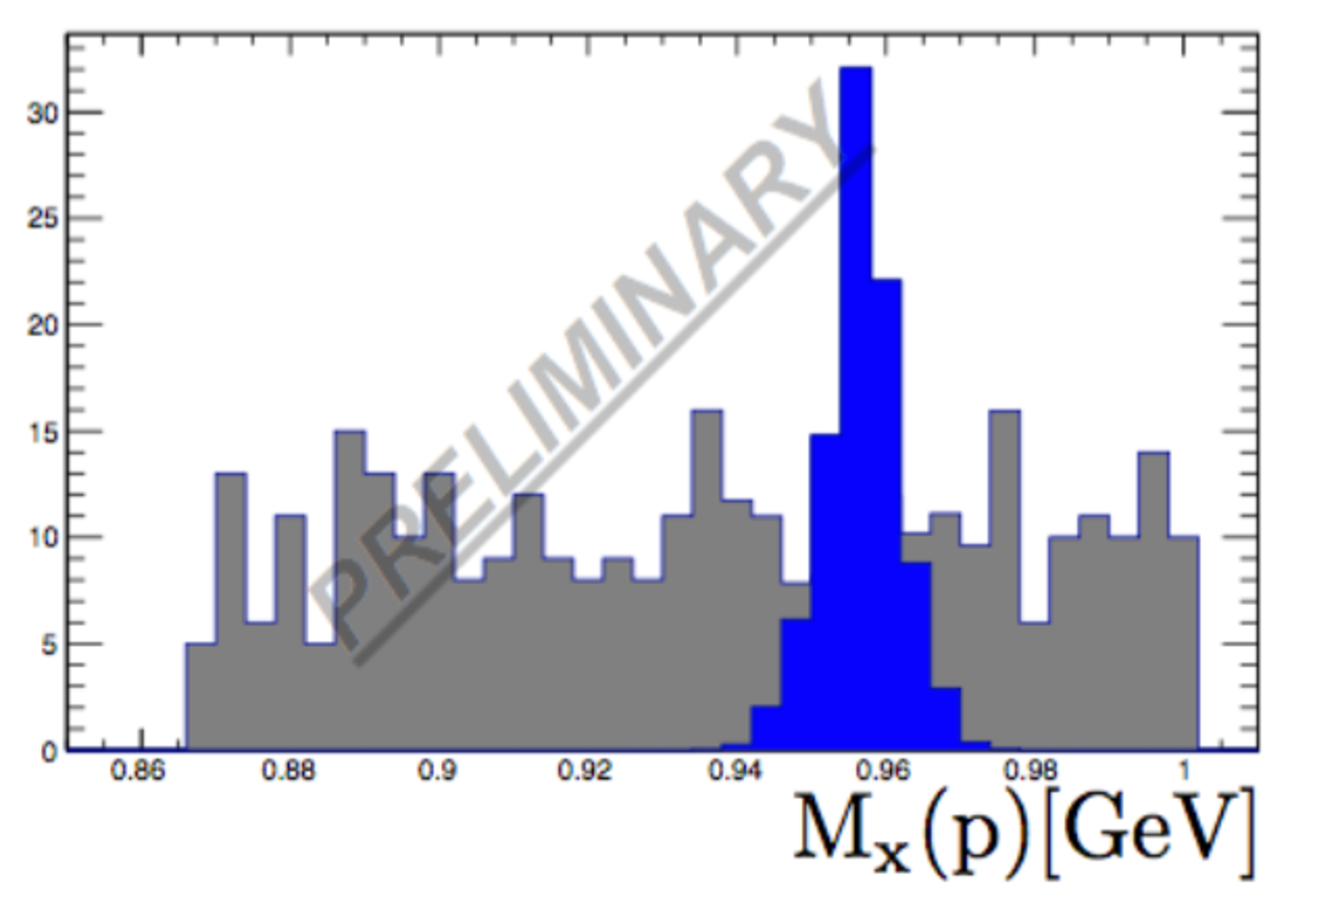
\includegraphics[width=160 pt]{figures/clas_etaP_ff_II.pdf}}
 	\caption{\textsc{\texttt{CLAS}} yield for $\gamma p \to p \eta^{\prime}  \to p e^+ e^- \gamma $ from g12 data set. Blue peak represents the signal extracted using the Q-factor method, while the gray band represents the background.}
 	\label{fig:etaP_ff}
 \end{figure}
  A preliminary branching ratio $\Gamma(\eta^{\prime} \to  e^+ e^-  \gamma)$/$\Gamma(\eta^{\prime} \to  \gamma  \gamma)$ was measured to be consistent with the BESIII measurement. However, the statistics of either BESIII or CLAS are not ample enough to determine, statistically, which theoretical model best represents the structure of the $\eta^{\prime}$ meson~\cite{bib10,bib11,bib12}. Table~\ref{tab:etaP.models} outlines the current measurements and theoretical predictions.
\begin{table}[h!]
\begin{minipage}{\textwidth}
\begin{center}


\caption{\label{tab:etaP.models}LMD planned measurements \vspace{0.75mm}}
\begin{tabular}{cc}
%\begin{tabular}{p{5cm} | p{7cm}}
\hline
Charge radius $\left< r\right>$ & Masurement (M) / Prediction (P) \\
\hline
CLAS ($\eta^{\prime}\to e^+e^-\gamma$)   & TBD \\
BESIII ($\eta^{\prime}\to e^+e^-\gamma$)   & (M) $1.60\pm0.17(stat)\pm0.08(sys) \mathrm{GeV}^{-2}$~\cite{bib7} \\
CELLO ($\eta^{\prime}\to \mu^+\mu^-\gamma$)   & (M)  $1.7\pm0.4 \mathrm{GeV}^{-2}$~\cite{bib9}  \\
Dispersion    & (P)  $1.53^{0.15}_{-0.08} \mathrm{GeV}^{-2}$~\cite{bib12}  \\
ChPT    & (P) $1.6 \mathrm{GeV}^{-2}$~\cite{bib11}  \\
VMD    & (P) $1.45  \mathrm{GeV}^{-2}$~\cite{bib10}  \\
\hline 
\end{tabular}


\end{center}
\end{minipage}
\end{table}
\vspace{20pt}
%
\subsection{Future Measurement of the $\eta^\prime$ Meson Transition Form Factor with \textsc{\texttt{CLAS12}}}
With the newly built \textsc{\texttt{CLAS12}} detector, $e^{\pm}$ identification can be achieved with a $e^{+}e^{-}/\pi^{+}\pi^{-}$ rejection of  $10^{6}-10^{11}$ while retaining $e^+ e^- \gamma$ acceptance $\sim 1 \% - 0.1 \%$, Figure~\ref{fig:clas12} depicts the \textsc{\texttt{CLAS12}} detector and its subsystems.
\begin{figure}[h!]
	\centerline{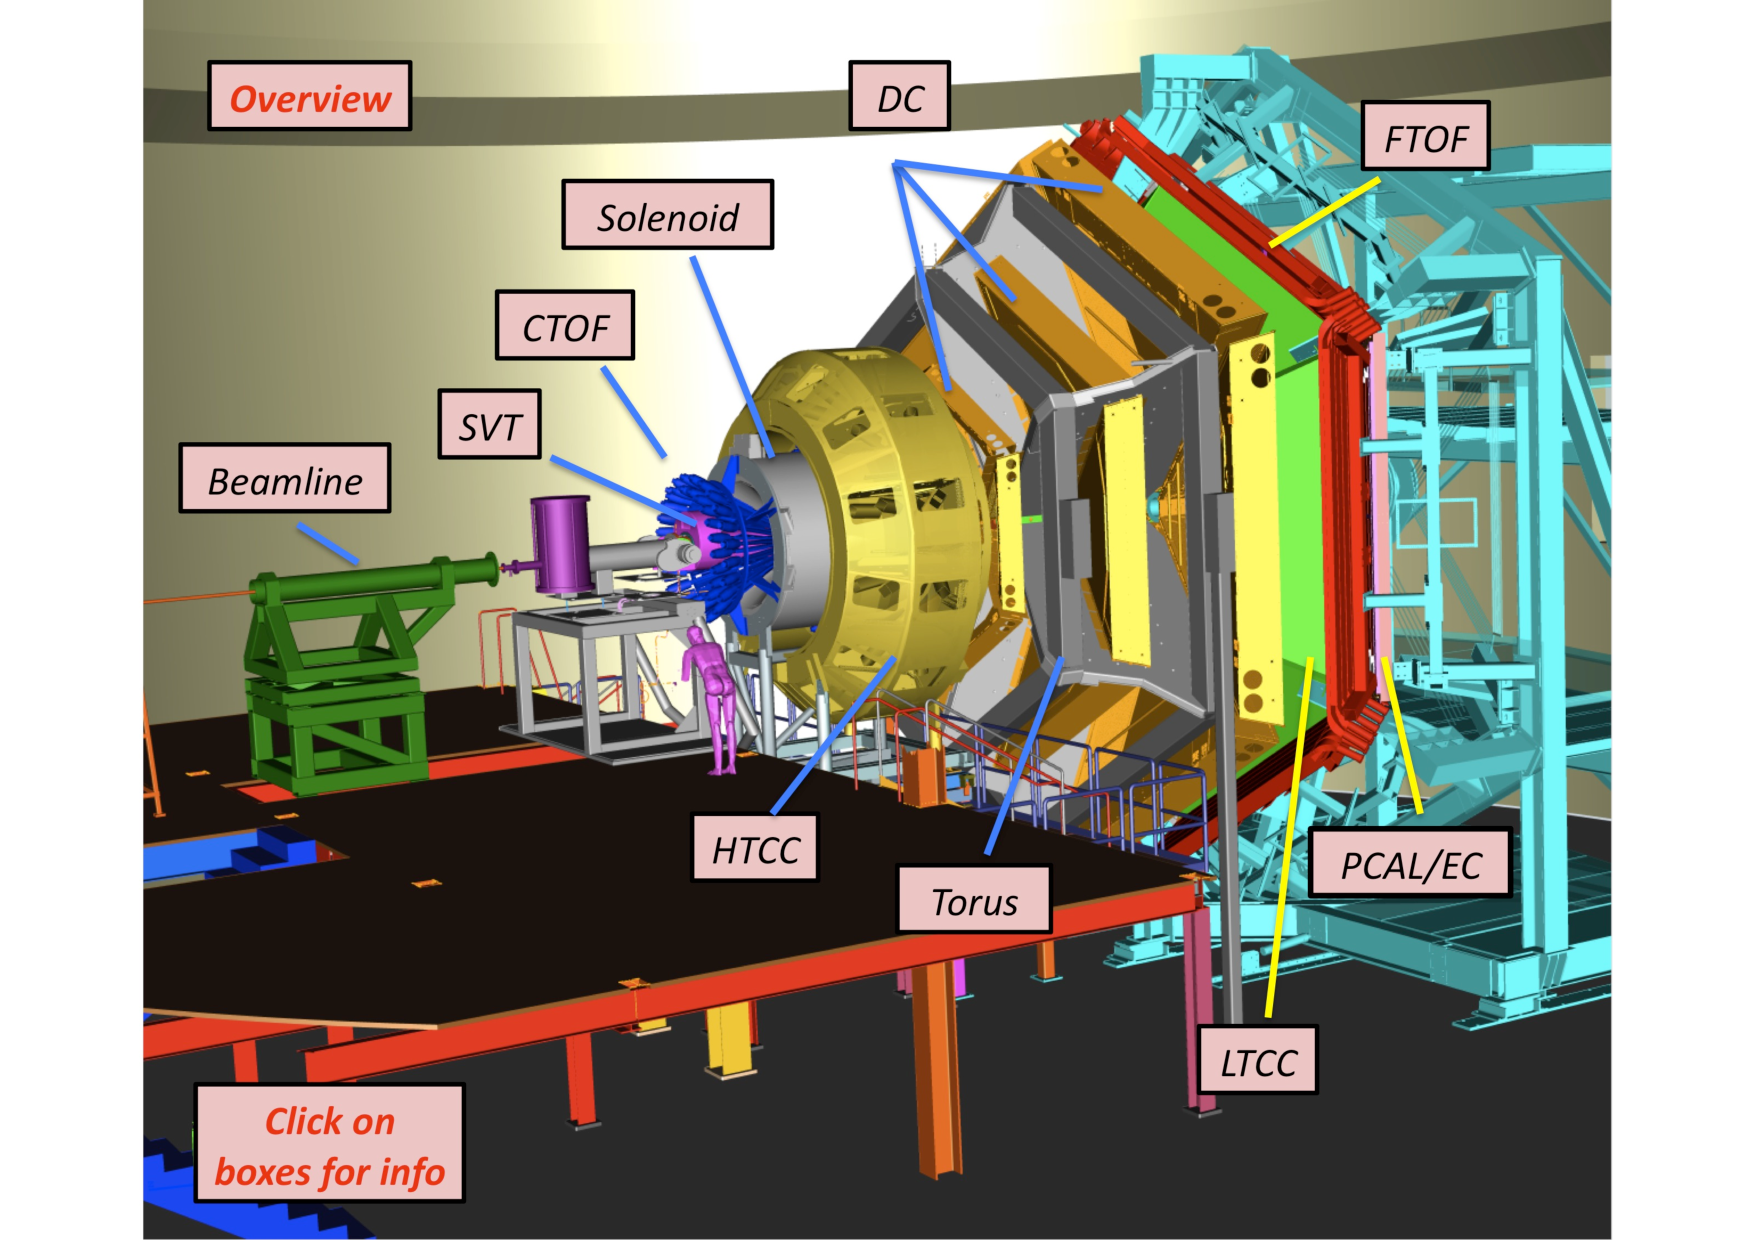
\includegraphics[angle = 90,width=250 pt]{figures/clas12-design.pdf}}
	\caption{The CEBAF Large Acceptance Spectrometer (\textsc{\texttt{CLAS12}})\\~(https://www.jlab.org/Hall-B/clas12-web/)}
	\label{fig:clas12}
\end{figure}
Using the GEant4 Monte-Carlo (GEMC) simulation suite for \textsc{\texttt{CLAS12}}, a simulation of 600,000 $e p \to e^{\prime} \gamma^* p \to p \eta^{\prime}  \to p e^+ e^- \gamma $ was performed. The generation of events included cross-section information obtained from previous \textsc{\texttt{CLAS}} measurements, the $s^n$ scaling law on the cross-section and the VMD model for the decay of the $\eta^{\prime}$ meson to achieve a reasonable model of the production of the $\eta^{\prime} $ meson. The estimated quasi-real photon rate with the \textsc{\texttt{CLAS12}} Forward Tagger are $5 \cdot 10^7 \gamma / s$ which will be impinged on  a 5~cm $\ell H_2$ target. Count rates of $ \eta^{\prime}  \to p e^+ e^- \gamma $ were calculated for exclusive $\gamma p \to p \eta^{\prime}  \to p e^+ e^- \gamma $ and inclusive $\gamma p \to \eta^{\prime} (p)  \to  e^+ e^- \gamma (p) $ with and without the electromagnetic calorimeter (EC) information for the $ e^+ e^- $ pairs. For the exclusive reaction it was preliminarily estimated that the number of  $ \eta^{\prime}  \to e^+ e^- \gamma $ decays to be detected within 100 days of beam time would be $\sim 22,000 - 2,400$, and the statistical uncertainty of the transition form factor measurement would be $\sim 0.3 \% - 3 \%$, with and without the EC information, respectively, Figure~\ref{fig:clas12_etaP}. For the inclusive reaction it was preliminarily estimated that the number of  $ \eta^{\prime}  \to p e^+ e^- \gamma $ decays to be detected within 100 days of beam time would be $\sim 53,000 - 5,900$, and the statistical uncertainty of the transition form factor measurement would be $\sim 0.1 \% - 1 \%$, with and without the EC information, respectively, Figure~\ref{fig:clas12_etaP}. Furthermore, with the statistics estimated to be seen in \textsc{\texttt{CLAS12}}, a $ \eta^{\prime} $ signal is expected in the complete range of $q = e^+ e^- $, allowing for a measurement at the divergent part of the VMD model $q\sim m_{\rho}$. 
%This will give greater insight into the structure of the $ \eta^{\prime} $ meson than previously measured. 
\begin{figure}[h!]
	\centerline{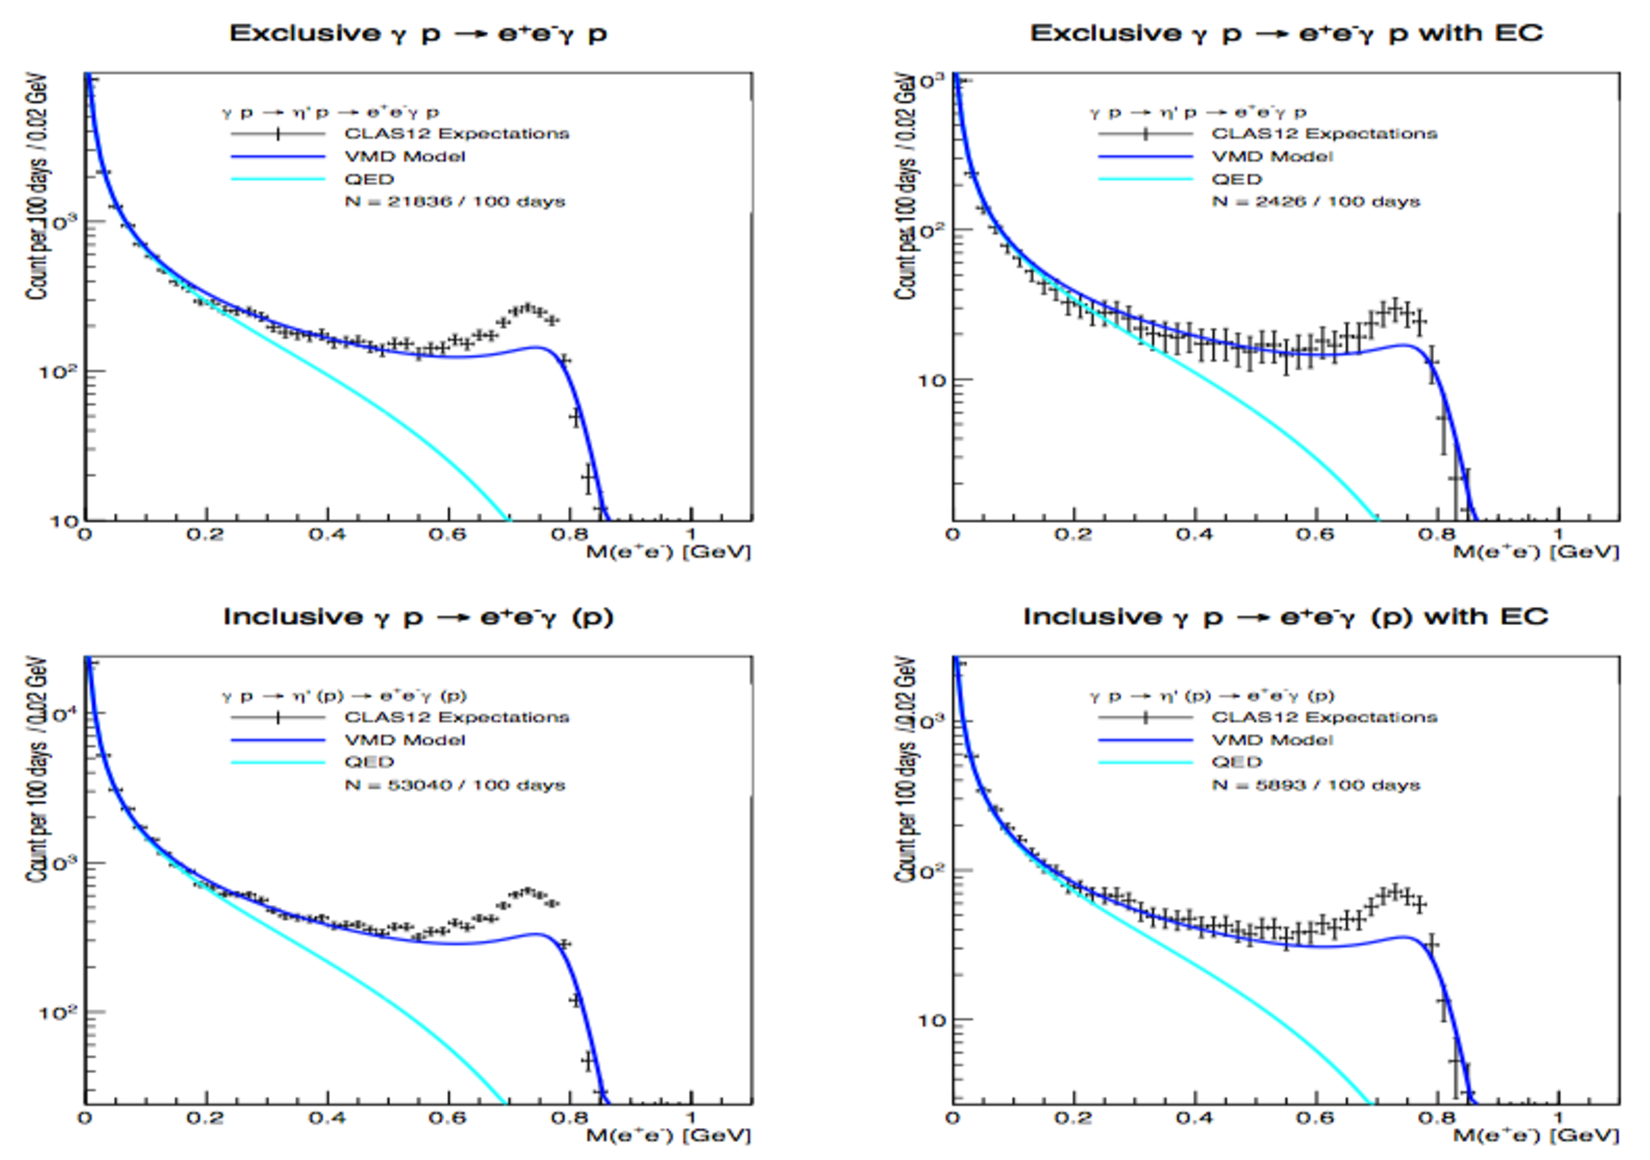
\includegraphics[width=350 pt, height=255 pt]{figures/clas12_etaP.pdf}}
	\caption{Expected count rates for $ \eta^{\prime}  \to e^+ e^- \gamma $ in \textsc{\texttt{CLAS12}}}
	\label{fig:clas12_etaP}
\end{figure}
%\begin{figure}[h]
%	\centerline{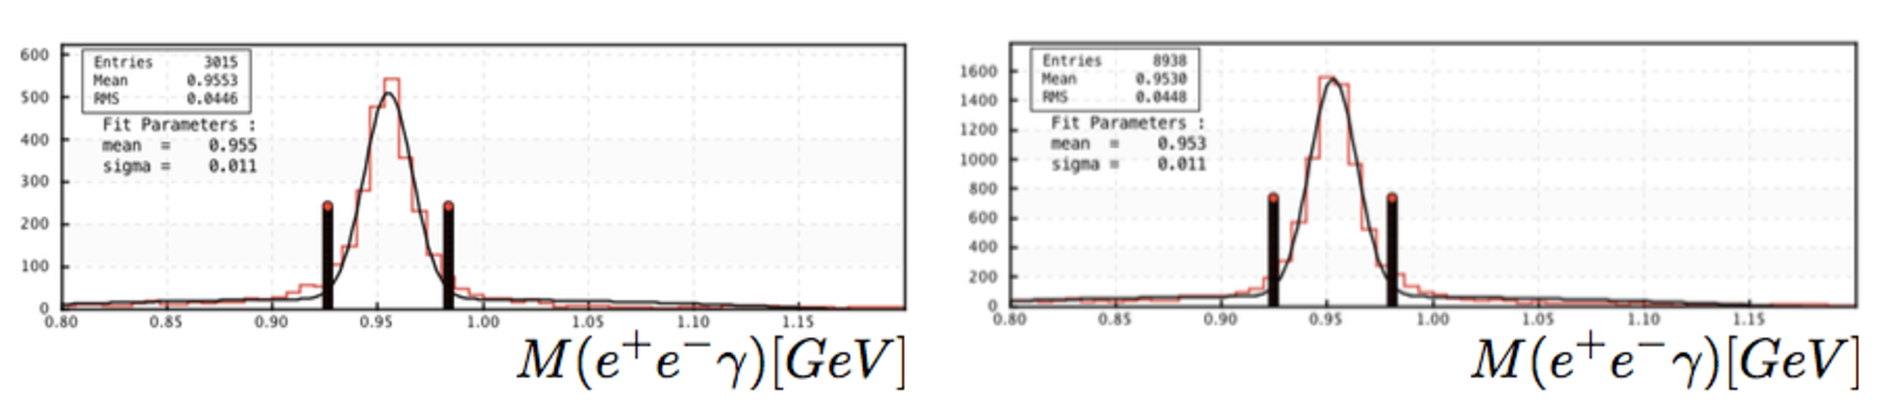
\includegraphics[width=200 pt, height= 100 pt]{figures/clas12_etaP_recon.pdf}}
%	\caption{The CEBAF Large Acceptance Spectrometer (\textsc{\texttt{CLAS12}})}
%	\label{fig:clas12_etaPrecon}
%\end{figure}
% Acknowledgement
%\section{ACKNOWLEDGMENTS}
%I would like to acknowledge the members of the LMD group for their contributions to the given presentation. Also to the CLAS collaboration.

% References

\nocite{*}
\bibliographystyle{aipnum-cp}%
\bibliography{LMD}%


\end{document}
